\section{Organisation d'un projet}

\begin{frame}
	\begin{center}
		\huge
		Organisation d'un projet
	\end{center}
\end{frame}

\subsection{Les modules} %%%%%%%%%%%%%%%%%%%%%%%%%%%%%%%%%%%%%%%%%%%%%%%%%%%%%%
\begin{frame}
	\frametitle{Principe des modules}
	\begin{center}
		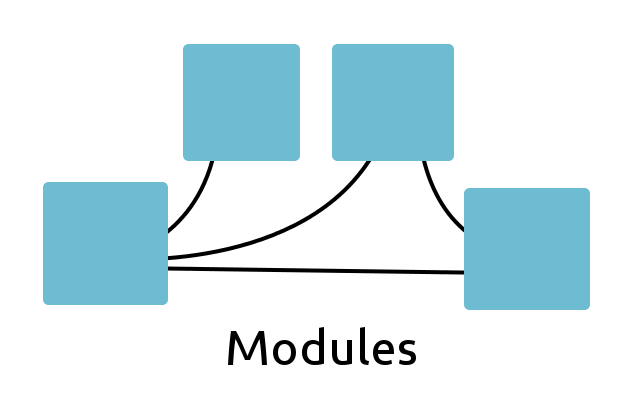
\includegraphics[width=9cm]{pics/modules.png}
	\end{center}
\end{frame}

\begin{frame}[fragile]
	\frametitle{Utilisation de fonctions d'un module}
	\begin{center}
		\begin{minipage}{0.5\textwidth}
			\begin{lstlisting}
open List

length 
  (1::3::3::7::[])
			\end{lstlisting}
		\end{minipage}
		\begin{minipage}{0.4\textwidth}
			\begin{lstlisting}
List.length 
  (1::3::3::7::[])
			\end{lstlisting}
		\end{minipage}
	\end{center}
\end{frame}

\begin{frame}
	\frametitle{Une facon de creer un module : Un fichier...}
	\begin{center}
		\begin{minipage}{0.5\textwidth}
			main.ml\\
			processing.ml\\
			rotation.ml\\
			cutting.ml\\
			recongition.ml
		\end{minipage}
		\begin{minipage}{0.4\textwidth}
			processing.mli\\
			rotation.mli\\
			cutting.mli\\
			recongition.mli
		\end{minipage}
	\end{center}
\end{frame}

\begin{frame}[fragile]
	\frametitle{Les fichiers surface}
	\begin{center}
		\begin{minipage}{0.34\textwidth}
			someFunctions.ml
			\begin{lstlisting}
let add a b = 
  a + b

let addf a b = 
  a +. b

let sub a b = 
  a - b

let subf a b = 
  a -. b
			\end{lstlisting}
		\end{minipage}
		\begin{minipage}{0.5\textwidth}
			someFunctions.mli
			\begin{lstlisting}
val add : 
  int -> int -> int

val addf : 
  float -> float -> float

val sub :
  int -> int -> int

val subf :
  float -> float -> float
			\end{lstlisting}
		\end{minipage}
	\end{center}
\end{frame}

\begin{frame}[fragile]
	\frametitle{Syntaxe d'un fichier interface 1/3}
	\lstset{basicstyle=\small}
	\begin{lstlisting}
val f : int -> int -> int

exception badSurface of (int -> int) * int

type card =
| Ace
| Number of int
| Head of HeadCard

type coloredPoint = {
  pos : int * int;
  mutable color;
}
	\end{lstlisting}
\end{frame}

\begin{frame}[fragile]
	\frametitle{Syntaxe d'un fichier interface 2/3}
	\lstset{basicstyle=\small}
	\begin{lstlisting}
class counter :
  object
    val mutable i : int
    method getCounts : unit -> int
  end

class point :
  int * int -> 
    object
      val pos : int * int
      method printCoord : unit -> unit
    end

class ['a] storage = 
  object val mutable data : 'a list method addData : 'a -> unit end
	\end{lstlisting}
\end{frame}

\begin{frame}[fragile]
	\frametitle{Syntaxe d'un fichier interface 3/3}
	\lstset{basicstyle=\small}
	\begin{lstlisting}
class ['a] storage = 
  object 
    val mutable data : 'a list
    method addData : 'a -> unit 
  end
	\end{lstlisting}
\end{frame}


\subsection{Faire de la documentation} %%%%%%%%%%%%%%%%%%%%%%%%%%%%%%%%%%%%%%%%
\begin{frame}
	\frametitle{La documentation}

\end{frame}

\begin{frame}
	\frametitle{ocamldoc}

\end{frame}

\begin{frame}
	\frametitle{La position des commentaires}

\end{frame}

\subsection{La compilation avec ocamlbuild} %%%%%%%%%%%%%%%%%%%%%%%%%%%%%%%%%%%
\begin{frame}
	\frametitle{Les differentes sorties d'OCaml}

\end{frame}

\begin{frame}
	\frametitle{Un Makefile rustique}

\end{frame}

\begin{frame}
	\frametitle{ocamlbuild}

\end{frame}

\begin{frame}
	\frametitle{Inclure des bibliotheques}

\end{frame}
